\section{编码与PIR的关系}
在传统的PIR协议中,编码一般用于多服务器PIR场景下。一种常见的场景是$t$-PIR,即客户端向多台服务器发送请求,允许其中$t$台服务器共谋,相互分享客户端发送的请求以尝试获取查询的信息。在这样的情况下,要求客户端查询索引保持隐私,不被泄漏。在此情景下,客户端可以对查询请求进行编码,以确保至少有$t+1$台服务器才能恢复出查询的内容。

然而,除了用于多服务器环境下的场景之外,编码还可以用于纠错\cite{10.1007/978-3-031-22368-6_3}。在像PIR这样的在线服务中,由于网络传输、硬件故障,甚至服务器受到恶意攻击等原因,查询错误是难以避免的。验证可以检测出错误,但无法从错误的结果中恢复正确的答案。在这些情境下,具有纠错功能的PIR协议更进一步地保障了PIR服务的可用性。

从计算与存储效率的角度来看,编码可以被视为数据库划分的一种扩展。编码允许我们将数据库划分为多个部分,每个部分存储在不同的服务器上,从而降低单台服务器的存储需求,充分利用多台服务器的计算能力。在这种情况下,选择编码不仅需要考虑编码的纠错能力,还需要考虑编码的空间利用效率。

\subsection{PIR中的数据库划分需求}
PIR与传统的数据库查询存在一个重要的区别:由于其对隐私性的要求,服务器接收的请求总是\textbf{缺乏局部性}的。这体现在以下两个方面:
\begin{enumerate}
    \item 在具有线性复杂度的PIR协议中,服务器总是需要在整个数据库上遍历以处理单个请求。
    \item 在具有亚线性复杂度的PIR协议中,服务器在处理请求时访问的记录是无法预测的。
\end{enumerate}

\begin{figure}
    \centering
    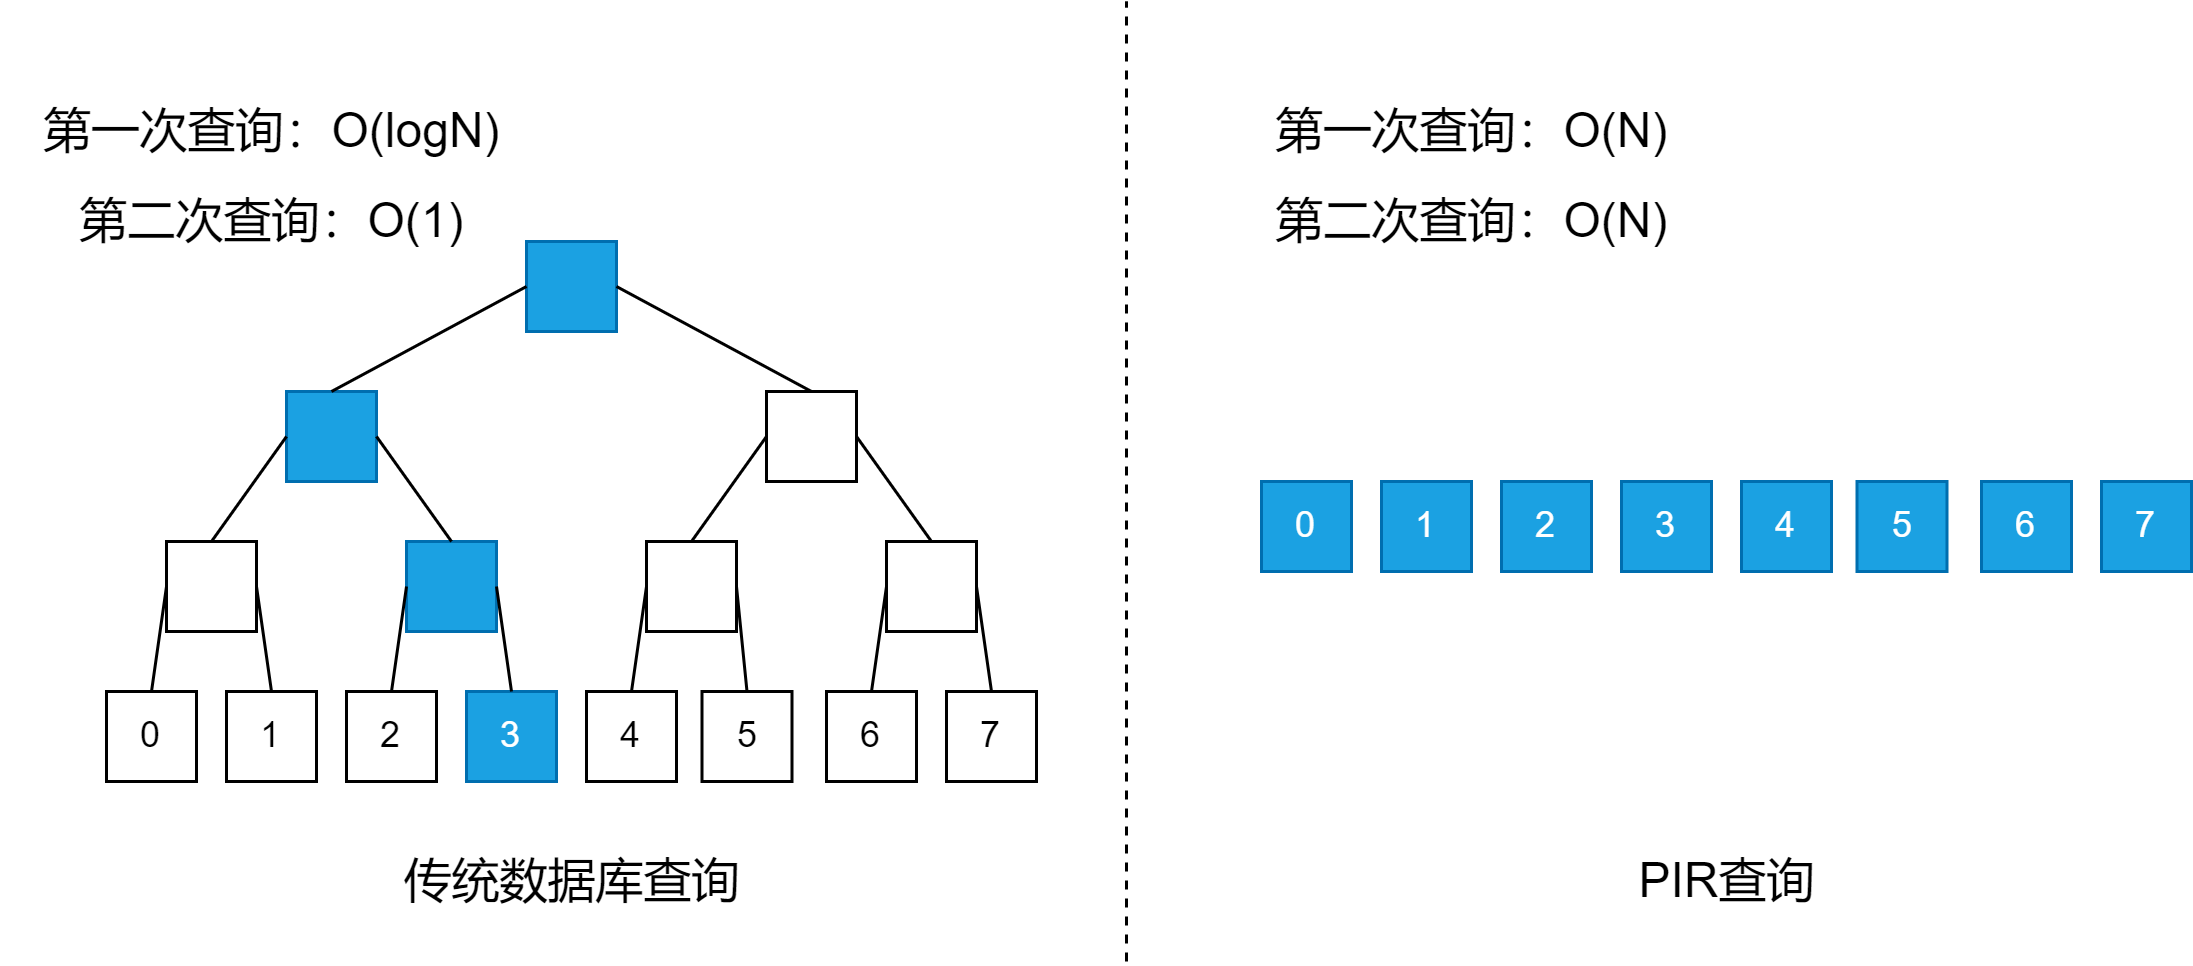
\includegraphics[width=0.8\textwidth]{figure/数据库模型.png}
    \caption{传统数据库与PIR模型对比}
    \label{fig:database-model}
\end{figure}

如图\ref{fig:database-model}所示,图中蓝色部分表示一次单点查询中被访问到的数据。在传统数据库中,如果利用数据库索引,单点查询的复杂度仅为对数级别。同时,通过缓存机制,后续的查询甚至可以避免访问数据库。然而,在PIR协议中,无论是利用索引还是缓存,都导致需要对所有记录进行运算,从而产生线性级别的复杂度。

这导致传统数据库中基于缓存和索引的查询加速机制无法直接应用于PIR。我们无法像传统数据库那样通过缓存查询结果来提高查询效率;同时,由于记录是线性存储在表中的,也无法利用索引快速访问特定记录。事实上,许多PIR协议\cite{SimplePIR,VeriSimplePIR,APIR,USENIX:KogCor21,EC:CorKog20,EC:CorHenKog22,MIR23}假设整个数据库都存储在内存中,而没有考虑从硬盘读取数据库内容的情况。然而,在实际应用中,这种假设是不合理的,因为数据库的大小可能超过单台服务器可用的内存总量。

\subsection{可验证PIR与纠错码}
一些研究探讨了将数据库划分后进行查询以提高效率\cite{RAID-PIR},但是在数据库划分之后,查询涉及的服务器数量增加,因此服务器集群中出现故障的可能性也相应增加。为了确保划分后数据库的可靠性,我们需要一种针对性的方法。

纠错码是一种常用于纠错的编码方式。如第\ref{sec:preliminary-code}节中所介绍的,纠错码通过在消息中添加冗余信息,使接收方能够检测并纠正错误。纠错码在解码时不要求知晓编码出错的位置,这与其一般应用场景一致——在普通消息传输中,无法单独验证每个码位的正确性。PIR协议可以利用纠错码,将编码后的数据库部署在多台服务器上。这时,每台服务器执行PIR查询的结果都是一个码位,即使有部分服务器出错,客户端只需获得足够多的码位即可获得查询结果。

在这种情况下,PIR查询的实际上是编码后的码位而不是数据库中的记录,这可能导致数据域的变化。由于本文提出的亚线性PIR协议不受此问题影响,因此此处不进行深入讨论。

在使用可验证PIR协议对每台服务器运行查询时,我们注意到,由于每个回答都可以单独验证,客户端事实上就获得了每个码位的正确性。因此,纠错码在这种情况下可以简化为纠删码。以Reed-Solomon编码为例,当作为纠错码时,其$(n, m, e)$编码方案通常需要满足$m = n + 2 \cdot e$。而当作为纠删码使用时,则只需要满足$m = n + e$。如果保持$m$和$n$的值不变(对应服务器总数和一次性编码的记录条数不变),那么$e$的值就会变为原先的两倍。这意味着进行简化后,相应的纠错阈值$t$将增加一倍。如果保持纠错阈值与服务器总数不变,那么每台服务器所承载的码位数量将减少。因此,即使纠错码能够验证服务器的答案,如果协议允许单独验证每个服务器的答案,协议的性能可以显著提高。

\label{sec:framework-assumption}
在进行数据库编码与分发这些任务时,需要进行协商或由中心协调人来完成,因此很难认为参与数据库划分的服务器之间不会共谋。因此,在本章提出的框架中,我们采用了一种最强的攻击模型,即假设所有服务器都由同一个实体控制。基于这一假设,我们提出了一个使用纠删码的PIR协议框架。